%convert -density 150x150 abra.pdf abra.png
\documentclass[margin=10pt]{standalone}
\usepackage{tikz}
\usetikzlibrary{arrows.meta, positioning}

\begin{document}
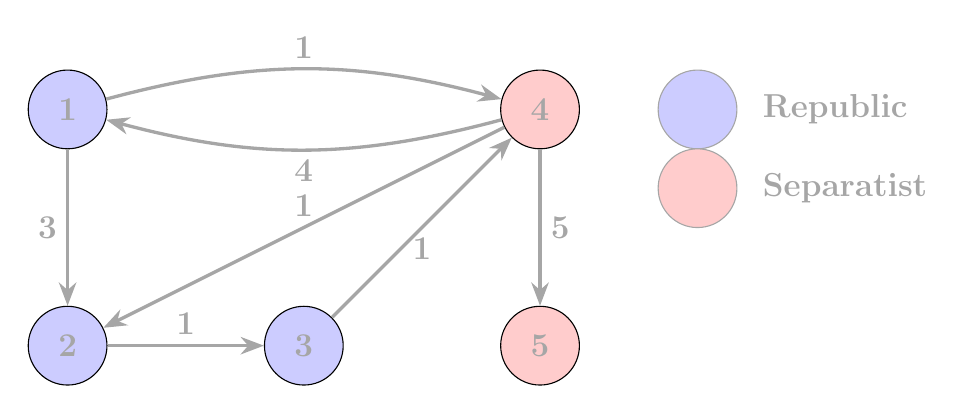
\begin{tikzpicture}[
    planet/.style={circle, draw, minimum size=1cm},
    republic/.style={planet, fill=blue!20},
    separatist/.style={planet, fill=red!20},
    edge/.style={->, very thick, >=Stealth, draw=gray!70},
    every edge label/.style={draw=none, font=\bfseries\small, text=gray!70},
    every node/.style={font=\large\bfseries, text=gray!70},
]

% Define planets (nodes)
\node[republic] (1) at (0,0) {1};
\node[republic] (2) at (0,-3) {2};
\node[republic] (3) at (3,-3) {3};
\node[separatist] (4) at (6,0) {4};
\node[separatist] (5) at (6,-3) {5};

% Define connections (edges) with distance labels based on updated input
\draw[edge] (1) -- node[midway, left, draw=none] {3} (2);
\draw[edge] (1) to[bend left=15] node[midway, above, draw=none] {1} (4);
\draw[edge] (2) -- node[midway, above, draw=none] {1} (3);
\draw[edge] (3) -- node[midway, below, draw=none] {1} (4);
\draw[edge] (4) -- node[midway, right, draw=none] {5} (5);
\draw[edge] (4) -- node[midway, above, draw=none] {1} (2);
\draw[edge] (4) to[bend left=15] node[midway, below, draw=none] {4} (1);

% Add a legend (moved up to the right of node 4)
\node[republic, draw=gray!70] at (8,0) (republ) {};
\node[right=0.2cm of republ, draw=none] {Republic};
\node[separatist, draw=gray!70] at (8,-1) (separ) {};
\node[right=0.2cm of separ, draw=none] {Separatist};

\end{tikzpicture}
\end{document}